%
% The MIT License (MIT)
%
% Copyright (c) 2016 Paul Batty
%
% Permission is hereby granted, free of charge, to any person obtaining a copy
% of this software and associated documentation files (the "Software"), to deal
% in the Software without restriction, including without limitation the rights
% to use, copy, modify, merge, publish, distribute, sublicense, and/or sell
% copies of the Software, and to permit persons to whom the Software is
% furnished to do so, subject to the following conditions:
%
% The above copyright notice and this permission notice shall be included in
% all copies or substantial portions of the Software.
%
% THE SOFTWARE IS PROVIDED "AS IS", WITHOUT WARRANTY OF ANY KIND, EXPRESS OR
% IMPLIED, INCLUDING BUT NOT LIMITED TO THE WARRANTIES OF MERCHANTABILITY,
% FITNESS FOR A PARTICULAR PURPOSE AND NONINFRINGEMENT. IN NO EVENT SHALL THE
% AUTHORS OR COPYRIGHT HOLDERS BE LIABLE FOR ANY CLAIM, DAMAGES OR OTHER
% LIABILITY, WHETHER IN AN ACTION OF CONTRACT, TORT OR OTHERWISE, ARISING FROM,
% OUT OF OR IN CONNECTION WITH THE SOFTWARE OR THE USE OR OTHER DEALINGS IN
% THE SOFTWARE.
%

\documentclass[a4paper,12pt]{article}

\usepackage{fancyhdr}						% for headers and footers.
\usepackage{setspace}						% for using single spaces.
\usepackage{mathptmx}						% for Times Roman Closest to Times New Roman.
\usepackage{listings}						% for code sections.
\usepackage{color}							% for colouring the code sections.	
\usepackage{graphicx}						% for images.
\usepackage{longtable}						% for large tables.
\usepackage{float}							% for floting points.
\usepackage{chngcntr}						% for numbering scheme
\usepackage[authoryear]{natbib}			% for refrencing.

\bibliographystyle{apalike}					% set refencing style
\bibpunct{(}{)}{;}{a}{,}{,}

\counterwithin{table}{section}				% set section number to caption for tables
\counterwithin{figure}{section}			% set section number to caption for figures

\hyphenpenalty 10000						% remove hyphenation at page width
\exhyphenpenalty 10000

\newlength{\wideitemsep}					% reduce the gap in lists
\setlength{\wideitemsep}{.5\itemsep}
\addtolength{\wideitemsep}{-7pt}
\let\olditem\item
\renewcommand{\item}{\setlength{\itemsep}{\wideitemsep}\olditem}

\makeatletter								% remove Refrence Title buit into biblatex.
\renewenvironment{thebibliography}[1]{
      \list{\@biblabel{\@arabic\c@enumiv}}
           {\settowidth\labelwidth{\@biblabel{#1}}
            \leftmargin\labelwidth
            \advance\leftmargin\labelsep
            \@openbib@code
            \usecounter{enumiv}
            \let\p@enumiv\@empty
            \renewcommand\theenumiv{\@arabic\c@enumiv}}
      \sloppy
      \clubpenalty4000
      \@clubpenalty \clubpenalty
      \widowpenalty4000
      \sfcode`\.\@m}
     {\def\@noitemerr
       {\@latex@warning{Empty `thebibliography' environment}}
      \endlist}
\makeatother

\pagestyle{fancy}							% use the fancy theme.
\fancyhead{}								% clear the headers.
\fancyfoot[CE,CO]{\leftmark}				% Put the Section into the footer.
\fancyfoot[LE,RO]{\thepage}					% put the page number into the footer.
\renewcommand{\headrulewidth}{0pt}			% remove the header rule / line.
\renewcommand{\footrulewidth}{0.4pt}		% place the footer rule / line.

\renewcommand{\arraystretch}{1.3}			% extra padding on tables.

\definecolor{dkgreen}{rgb}{0,0.6,0}		% define colours.
\definecolor{gray}{rgb}{0.5,0.5,0.5}		
\definecolor{mauve}{rgb}{0.58,0,0.82}
\definecolor{backcolour}{rgb}{0.95,0.95,0.92}
\definecolor{numbercolour}{rgb}{0.4,0.4,0.4}

\lstset{frame=tb,							% Set up code section settings.
  language=Java,							% language is java.
  aboveskip=3mm,							% top padding text.
  belowskip=3mm,							% bottom padding between text.
  showstringspaces=true,					% remove space characters.
  columns=flexible,							% flexible columns.
  basicstyle={\small\ttfamily},			% font.
  numbers=left,								% show line numbers on the left.
  numbersep=5pt, 							% size of line numbers.
  frame = false,							% remove the frame.
  backgroundcolor=\color{backcolour}, 		% set the colours.
  numberstyle=\tiny\color{gray},
  keywordstyle=\color{blue},
  commentstyle=\color{dkgreen},
  stringstyle=\color{mauve},
  numberstyle=\color{numbercolour},
  breaklines=false,							% don't break lines.
  breakatwhitespace=false,					% allow whitespace.
  tabsize=4									% set tab size.
}

\input{glyphtounicode}						% enable unicode.
\pdfgentounicode=1
\singlespacing								% enable single spaces.
\setlength{\parindent}{0cm}					% remove indentation.

\begin{document}
	%
% The MIT License (MIT)
%
% Copyright (c) 2017 Paul Batty
%
% Permission is hereby granted, free of charge, to any person obtaining a copy
% of this software and associated documentation files (the "Software"), to deal
% in the Software without restriction, including without limitation the rights
% to use, copy, modify, merge, publish, distribute, sublicense, and/or sell
% copies of the Software, and to permit persons to whom the Software is
% furnished to do so, subject to the following conditions:
%
% The above copyright notice and this permission notice shall be included in
% all copies or substantial portions of the Software.
%
% THE SOFTWARE IS PROVIDED "AS IS", WITHOUT WARRANTY OF ANY KIND, EXPRESS OR
% IMPLIED, INCLUDING BUT NOT LIMITED TO THE WARRANTIES OF MERCHANTABILITY,
% FITNESS FOR A PARTICULAR PURPOSE AND NONINFRINGEMENT. IN NO EVENT SHALL THE
% AUTHORS OR COPYRIGHT HOLDERS BE LIABLE FOR ANY CLAIM, DAMAGES OR OTHER
% LIABILITY, WHETHER IN AN ACTION OF CONTRACT, TORT OR OTHERWISE, ARISING FROM,
% OUT OF OR IN CONNECTION WITH THE SOFTWARE OR THE USE OR OTHER DEALINGS IN
% THE SOFTWARE.
%

\begin{titlepage}
	\begin{center}
		\begin{huge}
			\textbf{Continuous Deployment: A look at Architecture}
		\end{huge}	
		
		
		\vspace{3cm}		
		
		\normalsize By:   \\
		\large Paul Batty
		
		\vspace{2.5cm}
		
		\normalsize Supervisor: \\
		\large Manfred Lau
		
		\vspace{1.5cm}
		
		\large March 2017
		
		\vfill 
		
		\normalsize
		The dissertation is submitted to \\
		Lancaster University \\
		As partial fulfilment of the requirements for the degree of \\
		Integrated Masters of Science in Computer Science \\
	\end{center} 
\end{titlepage}

	%
% The MIT License (MIT)
%
% Copyright (c) 2017 Paul Batty
%
% Permission is hereby granted, free of charge, to any person obtaining a copy
% of this software and associated documentation files (the "Software"), to deal
% in the Software without restriction, including without limitation the rights
% to use, copy, modify, merge, publish, distribute, sublicense, and/or sell
% copies of the Software, and to permit persons to whom the Software is
% furnished to do so, subject to the following conditions:
%
% The above copyright notice and this permission notice shall be included in
% all copies or substantial portions of the Software.
%
% THE SOFTWARE IS PROVIDED "AS IS", WITHOUT WARRANTY OF ANY KIND, EXPRESS OR
% IMPLIED, INCLUDING BUT NOT LIMITED TO THE WARRANTIES OF MERCHANTABILITY,
% FITNESS FOR A PARTICULAR PURPOSE AND NONINFRINGEMENT. IN NO EVENT SHALL THE
% AUTHORS OR COPYRIGHT HOLDERS BE LIABLE FOR ANY CLAIM, DAMAGES OR OTHER
% LIABILITY, WHETHER IN AN ACTION OF CONTRACT, TORT OR OTHERWISE, ARISING FROM,
% OUT OF OR IN CONNECTION WITH THE SOFTWARE OR THE USE OR OTHER DEALINGS IN
% THE SOFTWARE.
%

\vspace*{\fill}

\begin{figure}[H]
	\raggedleft
	
\includegraphics[scale=1]{images/dec_head.jpg}
\end{figure}
\vspace{1cm}

\textbf{Name:} Paul Batty\\\\
\textbf{Student ID:} 33423253\\\\
\textbf{Dissertation Title:} Continuous Deployment: A look at Architecture.\\\\
\textbf{Module:} SCC.421 Fourth Year Project (Computer Science) \\\\

I certify that the material contained in this dissertation is my own work and does not contain unreferenced or unacknowledged material. I also warrant that the above statement applies to the implementation of the project and all associated documentation. Regarding the electronically submitted version of this submitted work, I consent to this being stored electronically and copied for assessment purposes, including the Department’s use of plagiarism detection systems in order to check the integrity of assessed work. I agree to my dissertation being placed in the public domain, with my name explicitly included as the author of the work.
\\\\\\
Date:
\\\\
Signed: 
\\\\\\\\

\begin{figure}[H]
	\raggedright
	
\includegraphics[scale=1]{images/dec_foot.jpg}
\end{figure}

\vspace*{\fill}

%\begin{center}
%To get the code and other documents visit the website at: 
%http://www.lancaster.ac.uk/ug/battyp/autotesting
%\end{center}
	%
% The MIT License (MIT)
%
% Copyright (c) 2017 Paul Batty
%
% Permission is hereby granted, free of charge, to any person obtaining a copy
% of this software and associated documentation files (the "Software"), to deal
% in the Software without restriction, including without limitation the rights
% to use, copy, modify, merge, publish, distribute, sublicense, and/or sell
% copies of the Software, and to permit persons to whom the Software is
% furnished to do so, subject to the following conditions:
%
% The above copyright notice and this permission notice shall be included in
% all copies or substantial portions of the Software.
%
% THE SOFTWARE IS PROVIDED "AS IS", WITHOUT WARRANTY OF ANY KIND, EXPRESS OR
% IMPLIED, INCLUDING BUT NOT LIMITED TO THE WARRANTIES OF MERCHANTABILITY,
% FITNESS FOR A PARTICULAR PURPOSE AND NONINFRINGEMENT. IN NO EVENT SHALL THE
% AUTHORS OR COPYRIGHT HOLDERS BE LIABLE FOR ANY CLAIM, DAMAGES OR OTHER
% LIABILITY, WHETHER IN AN ACTION OF CONTRACT, TORT OR OTHERWISE, ARISING FROM,
% OUT OF OR IN CONNECTION WITH THE SOFTWARE OR THE USE OR OTHER DEALINGS IN
% THE SOFTWARE.
%

\section*{\centering Abstract}

This paper looks into continuous deployment with a focus on the architecture of such a system from the ground up. Starting with where it came from, what it is and the technologies used. Then looking at what an ideal continuous deployment system would be all the way from developer to user. With a quick look at the cost-benefits and who would benefit from such a system. Then taking a look at what is missing, seeing that in general the tools and technology used is on the right track and destined for success. However, the embedded systems and continuous deployment seem to be out of sync therefore more tools need to be created to aid this area into being brought up to date with rest.

\vspace{1.5cm}

\textbf{Keywords:} Continuous deployment, Continuous integration, Automated builds, agile, VCS, workflow, Extreme programming 
	%
% The MIT License (MIT)
%
% Copyright (c) 2017 Paul Batty
%
% Permission is hereby granted, free of charge, to any person obtaining a copy
% of this software and associated documentation files (the "Software"), to deal
% in the Software without restriction, including without limitation the rights
% to use, copy, modify, merge, publish, distribute, sublicense, and/or sell
% copies of the Software, and to permit persons to whom the Software is
% furnished to do so, subject to the following conditions:
%
% The above copyright notice and this permission notice shall be included in
% all copies or substantial portions of the Software.
%
% THE SOFTWARE IS PROVIDED "AS IS", WITHOUT WARRANTY OF ANY KIND, EXPRESS OR
% IMPLIED, INCLUDING BUT NOT LIMITED TO THE WARRANTIES OF MERCHANTABILITY,
% FITNESS FOR A PARTICULAR PURPOSE AND NONINFRINGEMENT. IN NO EVENT SHALL THE
% AUTHORS OR COPYRIGHT HOLDERS BE LIABLE FOR ANY CLAIM, DAMAGES OR OTHER
% LIABILITY, WHETHER IN AN ACTION OF CONTRACT, TORT OR OTHERWISE, ARISING FROM,
% OUT OF OR IN CONNECTION WITH THE SOFTWARE OR THE USE OR OTHER DEALINGS IN
% THE SOFTWARE.
%

\section*{Introduction}
\label{sec:introduction}

Continuous deployment in no new idea as the field of computer science strives to automated all that it can. However, the idea and implementation of automating the development pipeline, going under the name of continuous integration and continuous deployment is a ever changing field. This has lead to the rise of devops also known as development operations dedicated to maintaining and building such systems with more of a focus on the collaboration of the different team involved in the pipeline such as quality assurance, development and management.
\\\\
During a recent project tasked with the aim to create the pipeline from the ground up there were many question that had to be answered. Such as what is the difference between continuous integration and continuous deployment. How does each part of the system fit into the big picture. What is the end game of the system. This is covered in the first section of this paper.
\\\\
Besides just understanding the reasoning and terms used behind the names, it was time to design and implement a system for the project. In addition to looking at the project that this idea spawned from, the paper will look at other attempts and experience from both industry and academic to understand the ideal architecture. This is covered in the second and third chapters.
\\\\
From here the paper will look at the how this architecture will work in practise, the patterns and the direction that this field is heading towards making sure that it is on the right track. This is covered in the final sections four and five.
\\\\
During the creation of the project there seemed to be no coherent or common meanings behind some of the terms. There also was a lack of architectural designs and implementations with most arguing about the systems cost-benefits.
\\\\
Therefore, the main aim of this paper is help define and understand the systems and terms used in this field. In addition to looking at the common themes used in practise to provide a guide for the creation of other automated systems, and those looking to understand this area more in depth.

	%
% The MIT License (MIT)
%
% Copyright (c) 2016 Paul Batty
%
% Permission is hereby granted, free of charge, to any person obtaining a copy
% of this software and associated documentation files (the "Software"), to deal
% in the Software without restriction, including without limitation the rights
% to use, copy, modify, merge, publish, distribute, sublicense, and/or sell
% copies of the Software, and to permit persons to whom the Software is
% furnished to do so, subject to the following conditions:
%
% The above copyright notice and this permission notice shall be included in
% all copies or substantial portions of the Software.
%
% THE SOFTWARE IS PROVIDED "AS IS", WITHOUT WARRANTY OF ANY KIND, EXPRESS OR
% IMPLIED, INCLUDING BUT NOT LIMITED TO THE WARRANTIES OF MERCHANTABILITY,
% FITNESS FOR A PARTICULAR PURPOSE AND NONINFRINGEMENT. IN NO EVENT SHALL THE
% AUTHORS OR COPYRIGHT HOLDERS BE LIABLE FOR ANY CLAIM, DAMAGES OR OTHER
% LIABILITY, WHETHER IN AN ACTION OF CONTRACT, TORT OR OTHERWISE, ARISING FROM,
% OUT OF OR IN CONNECTION WITH THE SOFTWARE OR THE USE OR OTHER DEALINGS IN
% THE SOFTWARE.
%

\section{Background}

The following chapter will cover two sections. Firstly, looking at where the idea for continuous development came from and the how the field ended up where it is today, going over the terms used. The second part looking at some of the tools used.

\subsection{History of Continuous deployment}

Continuous deployment is in a group of methodologies under the name of extreme programming (XP) which in turn is part of the Agile process \cite{XP}. The core principles of extreme programming is to be adaptive to change and quick feedback for everyone involved. Developers get feedback on the code, bugs and features. Clients get the features they need and Managers can make decisions about the direction of the project without bringing the whole system down. TODO:cite
\\\\
This movement started in March 1996 by Ken Back TODO:cite with continuous integration going further back to 1991 by Grady Booch TODO:cite. The main change between that of Booch's design and extreme programming, is that Booch placed a one integration a day limit, whereas extreme programming favours much more. TODO:cite
\\\\
The core idea behind Booch's idea is to avoid problems when a new release is integrated into an old system. It could achieve this goal via automated unit tests. Each test would run through a single public method and make sure that it is performing as it should. For example if a method takes two numbers and return the sum of the numbers. A unit test would test that \textit{1+1} will return \textit{2}, trying edge cases such as using letters and so on. In total there would be a group of tests for every public function. 
\\\\
After the developer has made a change to the code base they would run the tests if they all passed then the code was OK to be check in and used in the next release. This was enhanced with the idea of test driven development, where the test are written first then the change.
\\\\
This all started to kick off around 1997 with the continuous integration being place inside of the extreme programming movement.  This continued until 1999 through various books and publications by the movement, namely Kent Beck.
\\\\
Up to this point continuous integration just consisted of developers writing unit tests and running them locally to make sure that everything passes. When all the test pass the developer would then   check in the changes in to the version control system (VCS). Other developer then working on the same code base will be able to get the latest code and know that it works.
\\\\
This started to change around 2001 with the release of CruiseControl, because in the previous system what if a developer did not run the unit tests, or forgot or check in some files, so it would work fine on their local set-up but nowhere else. Therefore rather then leaving it up to the developer it could be automated. This introduced the idea of build servers. 
\\\\
A build server would sit there and depending on the particular set up and work-flow of the project,  would take the changes run the tests against them and then send out a report to the developer, or anyone who was interested. Now the if the developer forgot something it would be caught before anyone else started working on top of the changes.
\\\\
So far most of the work was performed by developers for developers, in order to assure that the current state of the code base was in a always working condition. This continues until 2008 when Patrick Debois and Andrew Shafer meet up and discuss bridging the gap between development, system administrators and other roles within the agile infrastructure. For example the developer environment is different to the test environment witch in turn is different to QA and production environments. 
\\\\
This then sparked the next stage in the movement, the creation of devops. This in turn created a whole host of new tools such as Jenkins (Hudson), Puppet and Chef just to name a few. These new tools made continuous integration easier then ever, and as they gained maturity started to see a lot of use in industry.
\\\\
As these tools started to gain popularity and with the internet being widespread, there was a shift to not only able to test, but as as the code is in a always working condition push out to the customers so they can always have the latest version, features and so on. This goes under the name of continuous deployment. This allows bugs to be fixed almost as quickly as they are found due to the reproduction of the customers environment back over in the developers workstation.
\\\\
Today, the transition over to continuous deployment is still being made, with more tools arriving. The idea of serverless severs and tools such as Docker in order to increase the reproducibility of the environments faster and with better accuracy.
\\\\
In short the entire pipeline is beneficial to everyone and comes in three different levels, automated builds, continuous integration and continuous deployment. Each being a step up from the one before it. 

\subsection{Tools}

In the previous part this paper named various tools that are used in the pipeline, they fall into three large categories, version control systems, testing  and infrastructure. In this next part the paper will look at each of the categories in turn to understand where they fit into the big picture and how they are used.

\subsubsection{Version control systems}

A version control system (VCS) or version control goes under two other names, revision control and source control. A VCS has a simple premise to manage the changes performed on a document. For example every time a document is edited, the changes are stored alongside the timestamp, user and other metadata. Then if at some point down the line a user want to see who made the changes or undo the changes as it broke the system they should be able to easily. 
\\\\
In short it is a system to manage a documents version, over long periods of time even when the system in closed, restarted or moved. This lays the foundations for more complex operations. As the changes are stored comparisons of different versions can be made, allowing them to be merged together.
\\\\
If user A sees an error in a document that the owner has not fixed, they can show the changes to the owner, if the owner agrees and likes the changes they can merge them in. This applies the changes from user A into the main document. This is also known as a pull request.
\\\\
If the owner makes a change to the document they do not need to send a pull request as they own the original, therefore they can merge right away. This merging is also called checking in, as the person is checking in there changes to the VCS.
\\\\
The VCS however, does not just record changes to just a single document but everything inside of a folder. Therefore it will track adding new files, deleting files and renaming files. Each VCS handles it slightly differently, however this is irrelevant to this paper.The folder will the in case of software development be the project root.
\\\\
If a VCS is tracking all files, then when checking in changes it would be a waste to do this per file, instead changes are grouped together under a commit. This commit is then checked in one go. Rather than a single file at a time, this allows relevant changes to be grouped together creating a nicer history for the project.
\\\\
VCS has one more main function to cover in respects to this paper, called branching. Similar to that in a tree VCS have a main or master branch called the trunk. A branch is similar to a workspace, and represents the changes on that workspace that got it to its current point.
\\\\
When branching it creates a copy of the current branch allowing it to take off in a different direction. Therefore development can go into two different directions without issues of people working on the same file. Then if needed can be merged back. This is better represented graphically as seen below in figure \ref{fig:vcs_branching}:

\begin{figure}[H]
	\centering
	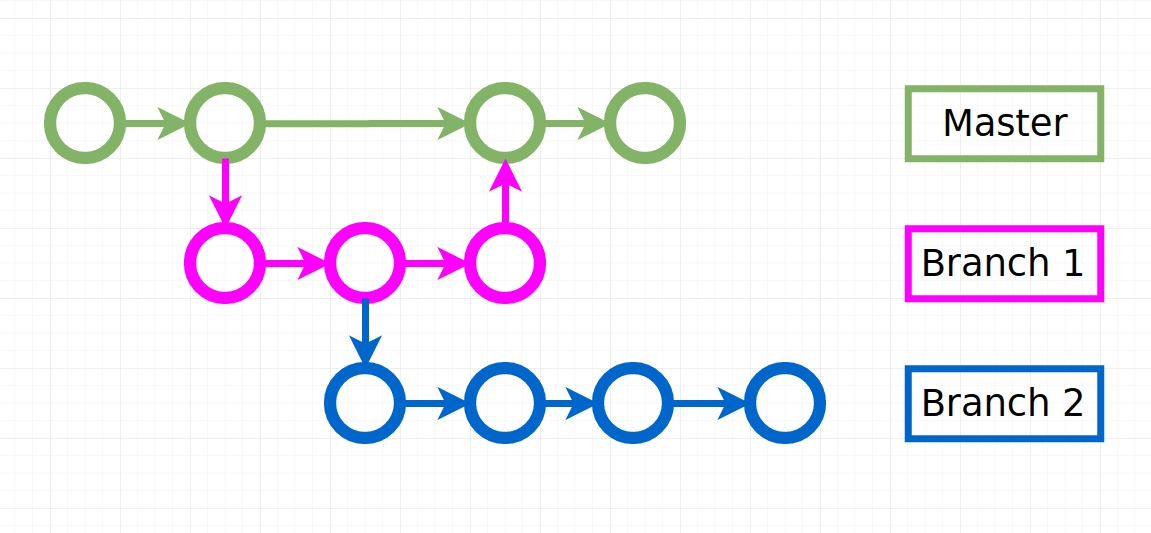
\includegraphics[scale=0.30]{images/branching.jpg}
	\caption{VCS Branching}
	\label{fig:vcs_branching}
\end{figure}

Each circle on the figure represents a commit (a group of changes). The figure also shows that branch one splits off from master, using it as its base then merged back in. While branch two uses branch one as its base, however has not yet been merged. There are different work-flows around this feature covered in more depth in section TODO:link the section.
\\\\
So far the paper has gone on about a folder that exists, this folder goes under the name of a repository. The next part will look at where the repository is located, such that multiple people or a single person can work on the project taking advantage of VCS, and how they differ. There are two main way that this is achieved, both use a client sever architecture. 
\\\\
The first has the server contain the repository, then the developer will create a local copy of the repository according to the branch they are on. They then work on the local copy editing files, however anything else such as creating a branch, merging or checking out files is performed by the server therefore a connection is required.
\\\\
The second way is distributed and has the developer create a local repository that mimic the server one then everything can be performed locally. When a connection to the server is available they can push their changes on the the server repository. This can be seen figure \ref{fig:vcs_systems}:

\begin{figure}[H]
	\centering
	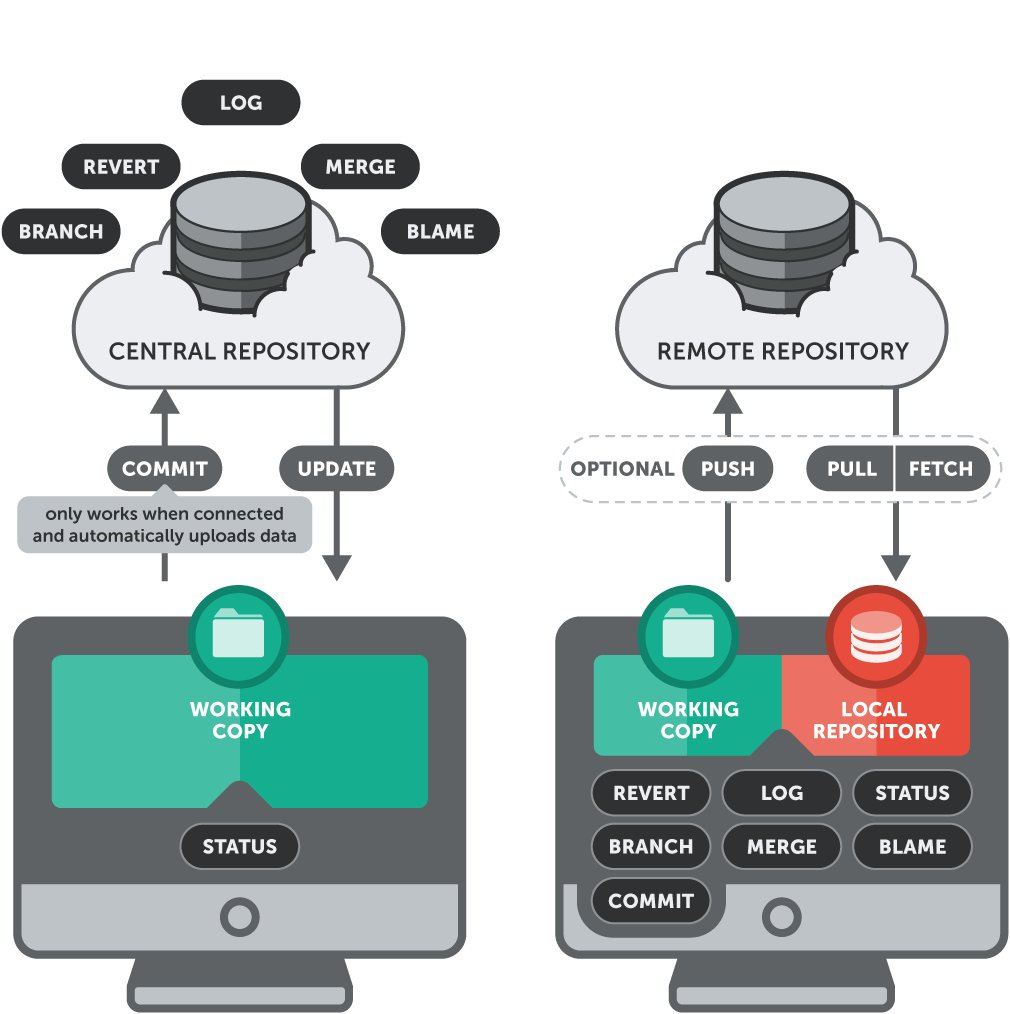
\includegraphics[scale=0.30]{images/systems.jpg}
	\caption{VCS systems modified from \cite{VCSSYSTEMS}}
	\label{fig:vcs_systems}
\end{figure}

There are a lot VCS out there, however the most popular is GIT, TFS and Subversion (\cite{vcspop}). Git follows the distributed system whereas TFS and Subversion uses the repository server system.
\\\\
There are a lot more intricate details to VCS however they will not be covered this paper.

\subsubsection{Testing}



\subsubsection{Infrastructure}
	%
% The MIT License (MIT)
%
% Copyright (c) 2017 Paul Batty
%
% Permission is hereby granted, free of charge, to any person obtaining a copy
% of this software and associated documentation files (the "Software"), to deal
% in the Software without restriction, including without limitation the rights
% to use, copy, modify, merge, publish, distribute, sublicense, and/or sell
% copies of the Software, and to permit persons to whom the Software is
% furnished to do so, subject to the following conditions:
%
% The above copyright notice and this permission notice shall be included in
% all copies or substantial portions of the Software.
%
% THE SOFTWARE IS PROVIDED "AS IS", WITHOUT WARRANTY OF ANY KIND, EXPRESS OR
% IMPLIED, INCLUDING BUT NOT LIMITED TO THE WARRANTIES OF MERCHANTABILITY,
% FITNESS FOR A PARTICULAR PURPOSE AND NONINFRINGEMENT. IN NO EVENT SHALL THE
% AUTHORS OR COPYRIGHT HOLDERS BE LIABLE FOR ANY CLAIM, DAMAGES OR OTHER
% LIABILITY, WHETHER IN AN ACTION OF CONTRACT, TORT OR OTHERWISE, ARISING FROM,
% OUT OF OR IN CONNECTION WITH THE SOFTWARE OR THE USE OR OTHER DEALINGS IN
% THE SOFTWARE.
%

\section{Evaluation}
\label{sec:evaluation}

eval
	%
% The MIT License (MIT)
%
% Copyright (c) 2017 Paul Batty
%
% Permission is hereby granted, free of charge, to any person obtaining a copy
% of this software and associated documentation files (the "Software"), to deal
% in the Software without restriction, including without limitation the rights
% to use, copy, modify, merge, publish, distribute, sublicense, and/or sell
% copies of the Software, and to permit persons to whom the Software is
% furnished to do so, subject to the following conditions:
%
% The above copyright notice and this permission notice shall be included in
% all copies or substantial portions of the Software.
%
% THE SOFTWARE IS PROVIDED "AS IS", WITHOUT WARRANTY OF ANY KIND, EXPRESS OR
% IMPLIED, INCLUDING BUT NOT LIMITED TO THE WARRANTIES OF MERCHANTABILITY,
% FITNESS FOR A PARTICULAR PURPOSE AND NONINFRINGEMENT. IN NO EVENT SHALL THE
% AUTHORS OR COPYRIGHT HOLDERS BE LIABLE FOR ANY CLAIM, DAMAGES OR OTHER
% LIABILITY, WHETHER IN AN ACTION OF CONTRACT, TORT OR OTHERWISE, ARISING FROM,
% OUT OF OR IN CONNECTION WITH THE SOFTWARE OR THE USE OR OTHER DEALINGS IN
% THE SOFTWARE.
%

\section{Conclusion}
\label{sec:conclusion}

At the start of the paper, several goals where defined. The first to look at and understand the terminology, history and meaning behind the various forms of continuous integration, continuous deployment and automatic build and the surround culture of devops. This was achieved in the first chapter of this paper.
\\\\
The second was to look at examples and other implementations of such system in the real world, taking a look at what went right, what they have in common and deriving the ideal systems from theses studies. This was achieved in the second and third chapters.
\\\\
Thirdly, to look at the cost benefits and who should use such as system in the first place, while looking at the status of the current situation around devops and where it is heading, making sure that it is on track. This took on the role looking at what is missing from the toolset and where thing have been done right.
\\\\
Overall, this project has been a success. The aims set out at the start have been achieved. There are a few minor issues that could be improved upon such as using more case studies to create a better foundation on which to draw from. 
\\\\
In the future, more time should be spend towards looking at creating easily reproducible and testing environments for embedded systems as they are non-existant when compared to the status of web, desktop and mobile development.
\\\\
But, this has been an enjoyable and successfully project and having learnt a great deal about the various technology stacks such as Docker, Vagrant and some of the more unique style of application such as serverless servers. In addition to a guide of which can be used when needed to implement a variation of  such a system
	%
% The MIT License (MIT)
%
% Copyright (c) 2017 Paul Batty
%
% Permission is hereby granted, free of charge, to any person obtaining a copy
% of this software and associated documentation files (the "Software"), to deal
% in the Software without restriction, including without limitation the rights
% to use, copy, modify, merge, publish, distribute, sublicense, and/or sell
% copies of the Software, and to permit persons to whom the Software is
% furnished to do so, subject to the following conditions:
%
% The above copyright notice and this permission notice shall be included in
% all copies or substantial portions of the Software.
%
% THE SOFTWARE IS PROVIDED "AS IS", WITHOUT WARRANTY OF ANY KIND, EXPRESS OR
% IMPLIED, INCLUDING BUT NOT LIMITED TO THE WARRANTIES OF MERCHANTABILITY,
% FITNESS FOR A PARTICULAR PURPOSE AND NONINFRINGEMENT. IN NO EVENT SHALL THE
% AUTHORS OR COPYRIGHT HOLDERS BE LIABLE FOR ANY CLAIM, DAMAGES OR OTHER
% LIABILITY, WHETHER IN AN ACTION OF CONTRACT, TORT OR OTHERWISE, ARISING FROM,
% OUT OF OR IN CONNECTION WITH THE SOFTWARE OR THE USE OR OTHER DEALINGS IN
% THE SOFTWARE.
%

\section*{References}
\label{sec:references}

\begin{thebibliography}{0}

% order aphabeticaly by first name.
\bibitem[Jong M. Deursen† A., 2015]{updatedatabse}
Jong M., Deursen† A. (2015), Continuous Deployment and Schema Evolution in SQL Databases, Delft University of Technology, Delft, The Netherlands
\\
\bibitem[Atlassian, 2017]{bamboo}
Atlassian. (2017), On line publication, Understanding the Bamboo CI Server, https://confluence.atlassian.com/bamboo/understanding-the-bamboo-ci-server\\-289277285.html, Last Accessed 23rd May 2017
\\
\bibitem[Berczuk S. Appleton B., 2002]{unit_tests}
Berczuk S., Appleton B. (2002), Software Configuration Management Patterns: Effective Teamwork, Practical Integration, Boston, ISBN 0201741172.
\\
\bibitem[Vassallo C. Zampetti F. Romano D., 2016]{CIF}
Vassallo C., Zampetti F., Romano D. (2016), Continuous Delivery Practices in a Large Financial Organization,In Proceedings of 2016 IEEE International Conference on Software Maintenance and Evolution, Raleigh, NC, USA, October 2 - 7, 2016, 519-528.
\\
\bibitem[Smith D., 2014]{XPH}
Smith D. (2014), On line publication, Extreme Programming (XP), http://projectmanagementhistory.com/Extreme\_Programming\_(XP).html, Last Accessed 22th May 2017
\\
\bibitem[Wells D., 1999]{XP}
Wells D. (1999), On line publication, Extreme programming: A gentle introduction, http://www.extremeprogramming.org/, Last Accessed 20th April 2017
\\
\bibitem[Engblom J., 2017]{intel}
Engblom J. (2017), On line publication, Continuous Delivery, Embedded Systems, and Simulation, https://software.intel.com/en-us/blogs/2017/03/13/continuous-delivery-embedde\\d-systems-and-simulation, Last Accessed 23rd May 2017
\\
\bibitem[Fournova Software, 2013]{VCSSYSTEMS}
Fournova Software. (2013), On line publication, Switching from Subversion to Git, https://www.git-tower.com/learn/git/ebook/en/command-line/appendix/\\from-subversion-to-git, Last Accessed 25th April 2017
\\
\bibitem[Fitz T., 2009]{deploy}
Fitz T. (2009), On line publication, Continuous Deployment for Downloadable Client Software, http://timothyfitz.com/2009/03/09/cd-for-client-software/, Last Accessed 23rd May 2017
\\
\bibitem[Hanna T., 2016]{cc}
Hanna T. (2016), On line publication, Comparing CI servers: Jenkins vs. CruiseControl vs. Travis, https://jaxenter.com/comparing-vi-servers-jenkins-vs-cruise-control-vs-travis-12\\5426.html, Last Accessed 22th May 2017
\\
\bibitem[Pepper K., 2013]{osspipeline}
Pepper K. (2013), On line publication, Automated Drupal Testing with Github Pull Requests, https://www.previousnext.com.au/blog/automated-drupal-testing-github-pull-re\\quests, Last Accessed 9th May 2017
\\
\bibitem[Fowler M., 2006]{mf}
Fowler M. (2006),  On line publication, Continuous Integration, https://martinfowler.com/articles/continuousIntegration.html, Last Accessed 22th May 2017
\\
\bibitem[Rapaport R., 2014]{devop_history}
Rapaport R. (2014), On line publication, A Short History of DevOps, https://www.ca.com/us/rewrite/articles/devops/a-short-history-of-devops.html, Last Accessed 22th May 2017
\\
\bibitem[Stackoverflow, 2017]{vcspop}
Stackoverflow. (2017), On line publication, Developer survey results, http://stackoverflow.com/insights/survey/2017\#work-version-control, Last Accessed 25th April 2017
\\
\bibitem[Karadzhov S., 2014]{zend}
Karadzhov S. (2014), On line publication, Fundamentals of Continuous Integration with Jenkins and zend server, http://static.zend.com/topics/WP-Fundamentals-of-Continuous-Integration-with\\
-Jenkins-and-Zend-Server-2014-03-31-EN.pdf, Last Accessed 4st May 2017
\\
\bibitem[Vaughan-Nichols S., 2014]{docker-vm}
Vaughan-Nichols S. (2014), On line publication, What is Docker and why is it so darn popular?, http://www.zdnet.com/article/what-is-docker-and-why-is-it-so-darn-popular/, Last Accessed 1st May 2017
\\
\bibitem[Mansoor U., 2016]{codeahoy}
Mansoor U. (2016), On line publication, Continuous Delivery - Automating the Release Process, https://codeahoy.com/2016/06/18/continuous-delivery-automating-the-release-\\process/, Last Accessed 5th May 2017
\\
\bibitem[Naik V., 2016]{thoughworks}
Naik V., (2016), On line publication, Architecting for Continuous Delivery, https://www.thoughtworks.com/insights/blog/architecting-continuous-delivery, Last Accessed 5th May 2017

\end{thebibliography}
	%
% The MIT License (MIT)
%
% Copyright (c) 2017 Paul Batty
%
% Permission is hereby granted, free of charge, to any person obtaining a copy
% of this software and associated documentation files (the "Software"), to deal
% in the Software without restriction, including without limitation the rights
% to use, copy, modify, merge, publish, distribute, sublicense, and/or sell
% copies of the Software, and to permit persons to whom the Software is
% furnished to do so, subject to the following conditions:
%
% The above copyright notice and this permission notice shall be included in
% all copies or substantial portions of the Software.
%
% THE SOFTWARE IS PROVIDED "AS IS", WITHOUT WARRANTY OF ANY KIND, EXPRESS OR
% IMPLIED, INCLUDING BUT NOT LIMITED TO THE WARRANTIES OF MERCHANTABILITY,
% FITNESS FOR A PARTICULAR PURPOSE AND NONINFRINGEMENT. IN NO EVENT SHALL THE
% AUTHORS OR COPYRIGHT HOLDERS BE LIABLE FOR ANY CLAIM, DAMAGES OR OTHER
% LIABILITY, WHETHER IN AN ACTION OF CONTRACT, TORT OR OTHERWISE, ARISING FROM,
% OUT OF OR IN CONNECTION WITH THE SOFTWARE OR THE USE OR OTHER DEALINGS IN
% THE SOFTWARE.
%

\section{Appendix}
\label{sec:appendix}
\end{document}